\documentclass[12pt,a4paper]{article}
\usepackage{setspace}
\usepackage[top = 1in, bottom = 1in, left = 1in, right = 1in]{geometry}
\usepackage[utf8]{inputenc}
\usepackage{amsmath}
\usepackage{amsfonts}
\usepackage{amssymb}
\usepackage{amsthm}
\usepackage{graphicx}
\usepackage{natbib}
\usepackage{caption}
\usepackage{subcaption}
\usepackage{float}
\usepackage{pdflscape}
\usepackage{booktabs}
\usepackage{dcolumn}
\usepackage{pdflscape}
\usepackage[hyphens]{url}
\usepackage{enumitem}
\usepackage[table]{xcolor}
\usepackage{authblk}
\usepackage{appendix}
\usepackage{titletoc}
\setlength\parindent{20pt}
\usepackage{setspace}
\usepackage{multirow}
\usepackage{caption}
\usepackage{titling}
\usepackage{amsmath}
\usepackage{hyperref}

\hypersetup{
    colorlinks=true,
    linkcolor=blue,
    filecolor=blue,      
    urlcolor=blue,
    citecolor=blue
}
\captionsetup[figure]{font=small,labelfont=small}

\DeclareMathOperator*{\argmax}{arg\,max}
\onehalfspacing
\usepackage[hang,flushmargin]{footmisc}

\newtheorem{theorem}{Theorem}[section]
\newtheorem{lemma}[theorem]{Lemma}
\newtheorem{proposition}{Proposition}
\newtheorem{corollary}{Corollary}
\renewcommand{\theproposition}{\arabic{proposition}}
\newcommand{\real}{\mathbb{R}_+^n}
\newcommand{\bfv}{\mathbf{v}}
\newcommand{\blue}{\textcolor{blue}}
% \renewcommand{\includegraphics}{\includegraphics[width=0.6\linewidth]}

\bibliographystyle{unsrtnat}

\title{Governing through patronage: the bargain for education in decentralized Brazil}
\date{\today}

\author{Galileu Kim}
\affil{Princeton University}

\begin{document}

\maketitle

\begin{abstract}
    How can governments improve the quality of education? I argue that local politicians govern through patronage, undermining education at the expense of voters. Building on qualitative evidence in Brazil, I leverage large-scale administrative data to show that public education is captured by local political elites. Mayors buy off local legislators to enact policy agendas by offering them positions into the educational sector. The degree to which patronage occurs varies: when mayors have a stronger ally base in the city council, they face less pressure to bargain. Patronage induces turnover in educational staff, with negative downstream effects on student learning. Weak electoral backlash suggest that patronage is primarily a political elite game, with limited accountability to the electorate. These findings point to the dangers of elite capture of public services and its downstream consequences for social welfare.
\end{abstract}

\newpage
\section{Introduction}

Across the world, vulnerable populations rely on governments for access to basic public services such as education. In the developing world, the quality of public education remains low: functional illiteracy is widespread, basic mathematical operations beyond the reach of most. This ``learning poverty'' is in  How can local governments improve the quality the of public services they deliver? In particular, how do political actors reshape bureaucratic institutions, and what are their downstream consequences for student learning.

To answer these questions, over two years I conducted fieldwork research in municipalities across Brazil. In interviews with local politicians, school principals and teachers, I discovered what many scholars working on the developing world already know: clientelism is pervasive, and it extends to public education with nefarious consequences \citep{stokes_brokers_2013}. However, the type of clientelism I observed was not embedded in electoral politics \citep{oliveros_making_2016} or partisan networks \citep{akhtari_political_2015,colonnelli_patronage_2017}, but the elite politics of government \citep{raile_executive_2011}. In Brazil, the exchange of public sector appointments for political favors -- a canonical example of patronage -- grants the mayor a carte blanche to enact her policy agenda.

In this paper, I argue that public education in municipalities across Brazil have been captured by political elites, with personnel appointments into public schools and management dominated by bargains between executive and legislative branches. Similar to coalition building in presidential contexts, mayors bargain for legislative support for their policy agenda through the allocation of public sector positions to city councilors and their constituencies \citep{laver_coalitions_1990, power_optimism_2010}. This effectively crowds out electoral accountability, as mayors prioritize building support by other political elites over voter welfare \citep{ferejohn_incumbent_1986}. By catering to the city council through patronage appointments, mayors shuffle the local educational bureaucracy, with negative downstream consequences for public school students.

The estimation proceeds in two parts. First, I show that political alignment between mayors and city councilors has a direct effect on patronage. Building on a canonical model of legislative vote-buying, I propose a theoretical model to analyze patronage under an institutionalized separation of powers, deriving my main empirical test: mayors who face less opposition in the city council engage in less patronage. To verify this hypothesis, I build a set of indicators to track educational staff turnover, leveraging administrative data of over 2 million school principals and teachers employed by municipalities. In line with qualitative accounts and theoretical expectations, mayors who have a stronger ally base in the legislature engage in less patronage. This results holds across a set of specifications and different measures of turnover.

I then show that this politically induced turnover has a negative impact on student learning. To estimate the effect of patronage on quality of education, I combine qualitative and quantitative evidence. Interviews conducted with educational bureaucrats and politicians suggested firm that turnover had a negative impact on teachers' ability to educate students, as time horizons were compressed and bonds between educators and learners were broken. To validate these accounts I combine administrative data on education from two separate student learning measures: \emph{Prova Brasil} and the \emph{SPAECE}. I construct multiple datasets to test these claims: the main specification contains over 1 million classrooms spread across the national territory. A set of estimations, combining multi-level modeling and fixed effects, provide strong evidence that teacher turnover has a negative effect on student learning.

This study contributes to an emerging literature on the politics of personnel and public services \citep{pepinsky_bureaucracy_2017, finan_personnel_2015}. I analyze how incentives shape political decision on how to manage local bureaucracies \citep{duflo_incentives_2012, gulzar_politicians_2017}, but I highlight the non-electoral policy goals of executive leaders. I also contribute to a growing research agenda on the consequences of political competition, demonstrating that increased political fragmentation between executive and legislative branches can lead patronage and decrease in the quality of public services. \citep{gottlieb_countervailing_2019, ferraz_corrupting_2012}. I bring to focus the end-to-end provision of public services, echoing a long-standing literature on state capacity \citep{kohli_state-directed_2004, evans_embedded_1995}.

The paper is structured as follows. Section \ref{sec:literature} provides an overview of the scholarly debate over public goods provision and personnel, as well as more specific treatments of the subject in Brazil. Section \ref{sec:context} presents the context and data. In section \ref{sec:theory}, I present the main argument, with a formal treatment of the subject using a canonical vote-buying model. Section \ref{sec:empirics} presents the research design and main results. Section 5 concludes.

\section{Related literature}
\label{sec:literature}

In this section I review extant literature on public goods provision and the politics underlying it, focusing on more recent studies of bureaucratic personnel and political leaders reshape these institutions. I also highlight how my research incorporates multiplicity in political actors and how this affects bargaining over public sector jobs. I address this gap by adapting previous analyses of executive-legislative bargaining to bureaucratic control at the local level.

\subsection*{Bureaucratic personnel and public goods provision}

Bureaucracies have a clear impact on the delivery of public services. A long-standing literature on state capacity provides a theoretical and substantive foundation to analyze bureaucratic institutions \citep{centeno_unpacking_2017, kohli_state-directed_2004}. A first generation of scholars, focusing on the successful developmental cases of East Asia, highlighted the need for a technocratic and autonomous bureaucracy \citep{johnson_miti_1982, kohli_state-directed_2004}. A Weberian wall separating bureaucrats from elected officials was considered indispensable for the successful provision of economic growth \citep{evans_bureaucracy_1999}.

Recent studies have added nuance to these claims, finding that high bureaucratic performance can coexist with political interference. Toral 2019 finds in Brazil that school principals appointed by mayors tend to perform better than their non-appointed counterparts in standardized test scores. \citet{gulzar_politicians_2017} show that local politicians who are able to internalize electoral benefits make bureaucrats exert more effort, increasing local employment. \citet{akhtari_political_2015}, on the other hand, highligh the pitfalls of political capture, showing that party turnover can lead to the replacement of school principals, with detrimental effects for student learning.

This recent wave of studies shed light on the intersection between politicians and bureaucracies. However, few of these studies explicitly model the multiple actors involved in managing bureaucracies. Understanding their diverse goals and action space provides a firm theoretical foundation to how different politicians can reshape bureaucracies. To do so I turn to the well-established literature on executive-legislative bargaining, applying its insights to the analysis of local government and administration.

\subsection*{Presidential coalitionism and patronage}

For every elected mayor in Brazil, a group of legislators are also elected into office. These political actors have competing claims over the local bureaucracy, with important implications for public service delivery. This structure parallels other settings with an institutinalized separation of powers and a bureaucratic pie to be split among the actors \citep{grindle_jobs_2012, mccarty_appointments_2004}. Divergent political interests can lead to strategic interaction between executive and legislative actors. A rich literature in Brazil explores these relations, with important insights to how executive and legislators bargain over bureaucracy. \citet{raile_executive_2011, power_optimism_2010}. 

In the Brazilian federal context, executive-legislative relations are analyzed under the prism of presidential coalitionism. Executive leaders garner legislative support from the National Congress by exchanging key positions in the federal bureaucracy, appointing members of their legislative coalition into cabinet positions. \citep{raile_executive_2011}. In a setting characterized by weak party cohesion and programmatic commitments \citet{ames_electoral_1995, lucas_ideological_2010}, bureaucratic positions for members of the coalition provide material incentives for legislators to support the executive agenda \citet{batista_o_2013, neto_presidential_2006, figueiredo_executivo_1999}.

In municipalities, mayors have to garner legislative support from city councilors to secure budgetary approval and implement desired policies. Due to weak programmatic commitments at the local level, public sector jobs are used to legislative support.\footnote{Interview with C, August and September 2019.} Mayors enjoy full discretion into how to appoint workers into the public sector, and use patronage to coopt legislative support from members of the coalition, a practice known locally as \textit{empreguismo}. As noted by a former mayor of the municipality of Sobral, "city councilors knocked on my door with a list of names for people they wanted me to hire."\footnote{Interview with C, August 2019.} These hires induce changes in personnel, with important consequences for bureaucracies and educational services.

\subsection*{Bureaucratic turnover and inexperienced education}

Bureaucracies exposed to turnover experience productivity shocks, often with detrimental effects. As new staff enters the bureaucracy, they must learn and acquire skills to deliver services to the population \citet{gailmard_slackers_2007}. Focusing on education, studies show that students taught by inexperienced teachers perform worse than those attending class with an experienced teacher \citet{clotfelter_teacher_2007}. \citet{akhtari_political_2015} finds that students attending a school with a recently appointed school principal perform worse in standardized test scores. When bureaucratic turnover is driven by patronage, political concerns take precedence over meritocratic ones \citet{colonnelli_patronage_2017}.

\begin{quote}
"I am aware that the position is temporary. Especially because it is a political position, decided by the administration. If the current administration is out of power, we are automatically dismissed." - Interview with school principal A, August 2019.
\end{quote}

Negotiations between executive and the legislative thus have a knock-on effect on the quality of educational services, as political considerations lead to bureaucratic turnover at the school and administrative level. In this study, the primary focus is on bureaucrats working within the boundaries of a school: school principals and teachers. In the following section I describe the institutional context for public education in Brazil, as well as the data employed for the the estimation.

\section{Institutional context and data}
\label{sec:context}

\subsection{Municipal education in Brazil}

In Brazil, the responsibility to provide public, primary education is primarily delegated to local governments \citet{paschoal_historia_2009}. In this critical learning period, students acquire skills such as reading/writing, as well as foundational concepts in math such as addition and substraction. The municipal educational system has increased in relevance over the past few decades, and currently over 60 percent of lower school strudents attend a public school. Figure \ref{fig:enroll} plots the total number of students in primary education per government level, including private schools. As of 2016, over 25 million students were enrolled in over 115 thousand municipal schools.

\begin{figure}[h]
    \centering
    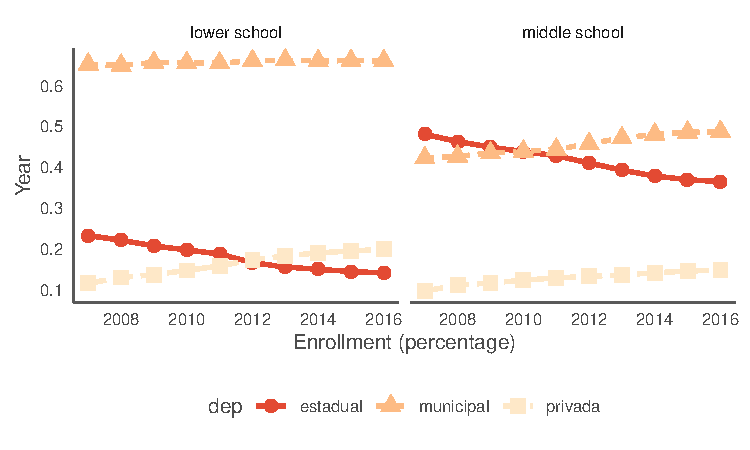
\includegraphics[width=0.6\linewidth]{plots/descriptive_enrollment.pdf}
    \caption{\textbf{Student enrollment by administration.}}
    \label{fig:enroll}
\end{figure}

The local executive branch has sole jurisdiction over the hiring and firing of teachers and school principals. School principals are considered positions of trust (\textit{cargos de confiança}) and usually appointed by the mayor or secretary of education \citet{brollo_victor_2017}. Teachers usually enter the public service through a public exam and are eligible for tenure after two years \citet{gatti_formacao_2010}. However municipalities increasingly resort to temporary contracts to hire new teachers as budgetary pressures amount. Municipal teachers and school principals are overseen by a local department of education \citep{militao_educacao_2014}.

Positions in the educational sector are politically valuable. As a department, it comprises over 25 percent of local public sector jobs. Due to their relatively high compensation and social status compared to other positions in the local bureaucracy, educational staff positions are particularly valuable for constituencies seeking employment. Additionally, qualitative evidence collected during fieldwork suggests that teachers play an important role in local party networks, leading electoral campaigns and brokering votes, similar to dynamics found by \citet{oliveros_making_2016} in Argentina's campaigning teachers.

\begin{figure}[h]
    \centering
    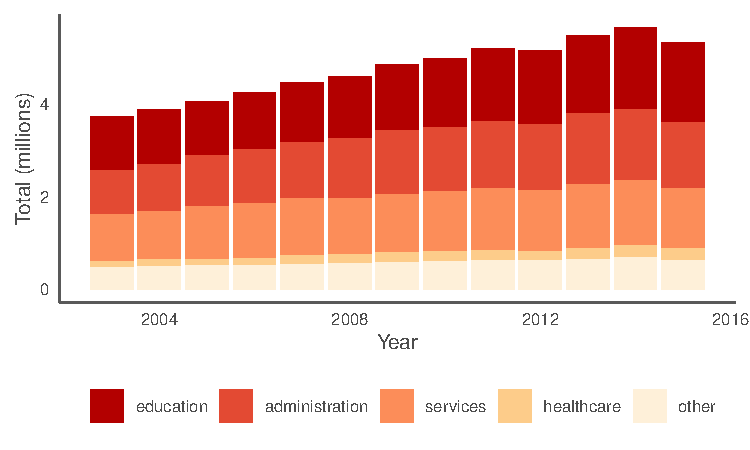
\includegraphics[width=0.6\linewidth]{plots/descriptive_staff_breakdown}
\end{figure}

Funding for municipal education relies primarily on federal transfers, the Fundeb, derived from 10 percent of tax revenues for each level of government to education. At the municipal level, 25 percent of the local budget must be allocated to education, and compensatory federal transfers are institutionalized by law to those municipalities which do not reach the target.\footnote{For more details on the Fundeb, see \hyperlink{https://www.fnde.gov.br/index.php/financiamento/fundeb/sobre-o-plano-ou-programa/sobre-o-fundeb}{here}}. While municipalities may be audited to verify whether funds are being properly used, personnel decisions and daily operations are fully under municipal discretion \citet{ferraz_corrupting_2012}.

\subsection{Local governance and mayoral coalitions}

Brazil's local level government is composed by over 5 thousand municipalities, each with their own mayor hall (\emph{prefeitura}) and city council (\emph{c\^{a}mara dos vereadores}). Mayors and city councillors (\textit{vereadores}) are democratically elected every four years, with the possibility of reelection for both.\footnote{The last municipal elections were in 2016. These take place every 4 years.} The executive is responsible for the management of public services such as education, with exclusive rights over personnel apppointment. The city council, on the other hand, oversees legislation and approves the budget for the fiscal year. As noted by \citet{souza_reforma_2004}, decisions over whom to appoint into the educational sector are primarily in the hands of the mayor and her secretary of education.

In order to win elections and garner support for their campaign, mayors form electoral alliances with local party labels \citet{dantas_eleicoes_2013}. These mayoral coalitions, once in government, are an important basis for approving budgets and, more generally, executive control over the legislative chamber. Interviews with city councilors indicate that the legislature is divided into a pro-government (\textit{governo}) and opposition (\textit{oposição}) groups (\textit{bancada}). While these electoral coalitions do not necessarily remain intact once governments are formed, fragmentation is generally on the margins, with mayors swapping defecting legislators for new ones.\footnote{Interview with C, former chief of staff of municipality J. September 2018.}

Interviews with secretaries of education and mayors provide evidence that city councilors play an important role in staffing decisions. While mayors hold jurisdiction over personnel decisions, there are extensive consultations between mayors and city councilors to decide who becomes the principal of a school, or which teacher remains in a school or leaves. These executive-legislative consultations ultimately determine the allocation (\textit{alotação}) of educational staff, serving as the primary tool through which mayors reward or coopt legislators into supporting them in the city council. In the words of a set of school administrators in the municipality of I:

\begin{quote}
    \emph{School principal}: Here, we are invited to work at the school by the department of education, with the [political] candidate, the city councilor...deciding which are the positions they are searching for and appointing people they think have the necessary qualifications.

    \emph{Educational counselor}: I was also invited to work here, by the city councilor and the department of education.\footnote{Interview with the administrative board of school A., municipality J. August 2019.}
\end{quote}

These accounts, along with previous case studies of municipalities in Brazil, suggest that city councilors play an important role in nominating staff. To verify these claims in a broader set of municipalities, as well as outlining the research design, I apply a theory of legislative vote-buying that illustrates the  employ extensive administrative and electoral data collected by the Brazilian federal government. In the next section I describe the data, where it is publicly available, as well as the preparation necessary for the set of estimations presented in the study.

\subsection{Data}

Brazil collects fine-grained data on education and makes it publicly available for research. For this study, data on education are collected from two main sources: the SAEB and School Census.\footnote{These can be accessed \hyperlink{http://portal.inep.gov.br/web/guest/dados}{here}.} The SAEB (National System for Educational Assessment) is a biannual standardized exam administered by the INEP (National Institute fosr Educational Studies and Research) to all public schools and a sample of private schools. In 2017, over 5 million students, in 5th and 9th grade, took the exam, testing their proficiency in both mathematics and Portuguese. In this study, test scores are the primary metric for assessing the quality of education received by students.

\begin{figure}[h]
    \centering
    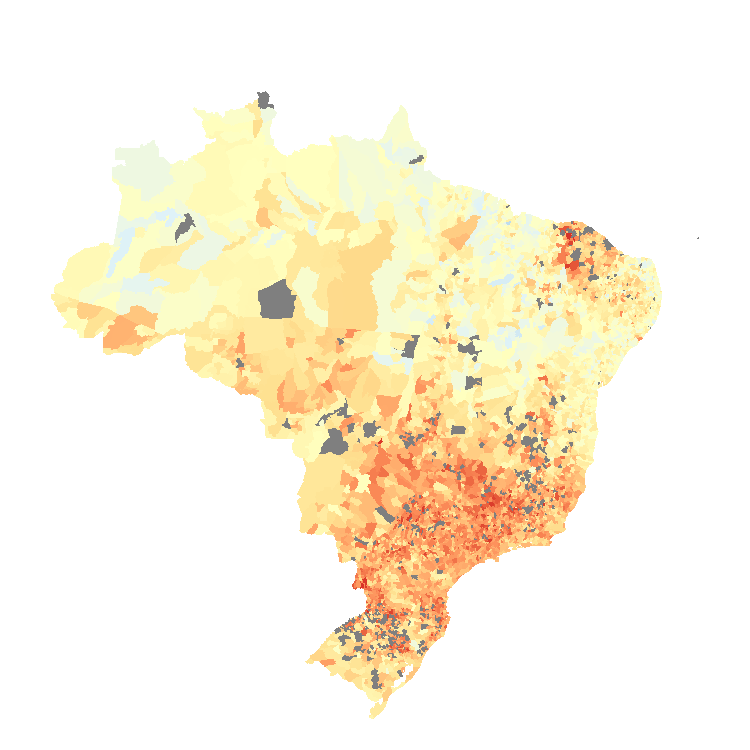
\includegraphics[width=0.6\linewidth]{plots/saeb_map.pdf}
    \caption{Uneven quality of municipal education. Polygons represent municipalities, warmer colors indicate higher municipal average in standardized test scores. Averages are weighted by student participation rate.}
    \label{fig:saeb_map}
\end{figure}

Figure \ref{fig:saeb_map} presents a map of Brazil with the municipal averages for the SAEB of 2015. Warmer colors such as red and orange indicate higher average scores, with the converse denoted by colder, blue shades. There is clear variation in average test scores, with the Southeast and Midwest outperforming poorer regions in the North and Northeast. Even within regions, however, there is wide heterogeneity. In particular, note that in the northern part of Brazil, high-performing municipalities neighbor low-performing ones. This indicates that despite spatial clustering, municipal factors can lead to variation in the quality of education.

Employment data on educational staff, including teachers and school principals, are extracted from the RAIS, SAEB and the School Census.\footnote{RAIS data, along with additional Brazilian employment data, can be accessed \hyperlink{http://trabalho.gov.br/dados-abertos}{here}.} The \emph{Relatório Anual de Informações Sociais} (RAIS) is an annual census administered by the now Ministry of Finance to all formal employers in Brazil. Employers are mandated to accurately report data on employees, subject to fines for misreporting. Subnational governments, including municipalities, also report to the RAIS. The dataset therefore contains micro-level information on all municipal personnel, including when they were hired/fired, as well as wages, type of contract and education levels.

Figure \ref{fig:staff_turnover} provides descriptive statistics on bureaucratic personnel in Brazil, segmented by department. Educational staff, in this case school principals and teachers, comprise approximately a third of municipal public sector jobs, totaling around 2 million in 2015. While comparable to administrative staff, this total significantly exceeds that for healthcare services. Focusing on turnover, we note that new hiring and dismissals in education staff is relatively high. While lower than that for administrative staff, new hires can represent over 10 percent of extant staff. The past two decades was a moment of rapid expansion of municipal staff, and hiring has far exceeded dismissals in that time period.

\begin{figure}[h]
    \centering
    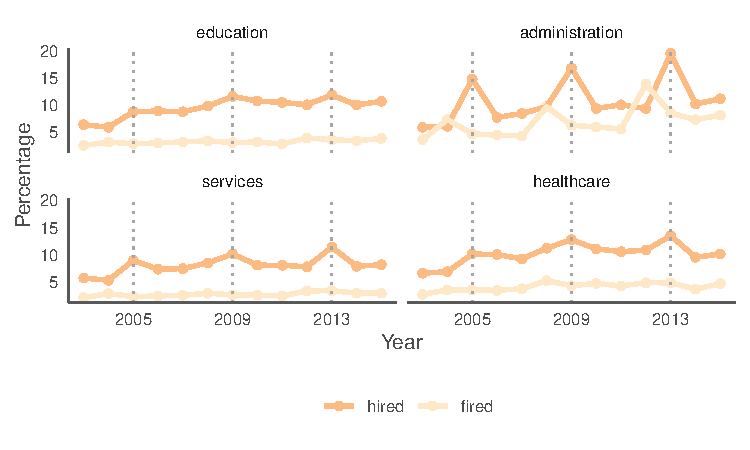
\includegraphics[width=0.\linewidth]{plots/descriptive_staff_turnover.pdf}
    \label{fig:staff_turnover}
    \caption{Proportion of public sector jobs by department. Note that I only keep the top 5 categorie}
\end{figure}

I propose three different specifications for measuring bureaucratic turnover. From the RAIS I obtain the percentage of teachers and principals who are dismissed and hired at any given year. Using school census data, it is possible to track individual teachers across time and schools. With that data I calculate a turnover index for school $s$, in municipality $j$ at year $t$, based on an index proposed by \citet{pereira_junior_indicadores_2016}. The number of teachers leaving and entering the school at a given year are summed and divided by the total number of teachers in the current and previous period.

$$\text{turnover}_{sjt} = \frac{\text{exit}_{sjt} + \text{entry}_{sjt}}{N_{sjt} + N_{sjt-1}}$$

\blue{Insert more information and descriptive paragraph on turnover index here}

Information on mayor, city councilors and mayoral coalitions are made available by the Supreme Electoral Court (TSE), the national authority responsible for overseeing elections.\footnote{Available \hyperlink{http://www.tse.jus.br/eleicoes/estatisticas/repositorio-de-dados-eleitorais-1}{here}.} In order to calculate the share of legislative seats held by the mayoral coalition, I match the partisanship of each city councilor to the mayoral electoral coalition. The distribution of share of coalition seats is depicted in figure \ref{fig:hist_coalition}. Note that although most city councils are controlled by the mayor, in over 40 percent of municipalities the mayoral coalition is a minority government.

\begin{figure}
    \centering
    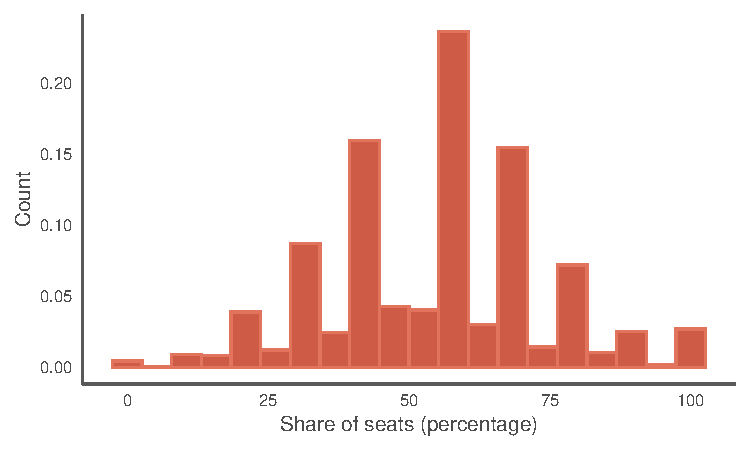
\includegraphics[width=0.6\linewidth]{plots/hist_coalition.pdf}
    \caption{Distribution of share of legislative seats allied with the mayor during the electoral campaign for the elecoral period of 2002-2016.}
    \label{fig:hist_coalition}
\end{figure}

Additional data has been collected to supplement the estimation exercise. Sociodemographic data comes from the National Institute for Statistics and Geography (IBGE), budgetary data from (FINBRA) and student test scores from Ceará (SPAEEC) are graciously provided by the Department of Education of Ceará.\footnote{Respectively, data can be found here: (1)\hyperlink{https://ces.ibge.gov.br/base-de-dados/links-base-de-dados.html}{IBGE}, (2)\hyperlink{https://siconfi.tesouro.gov.br/siconfi/pages/public/consulta_finbra/finbra_list.jsf}{Finbra}, (3)\hyperlink{https://www.seduc.ce.gov.br/spaece/}{Spaece}.}

\section{Theory}
\label{sec:theory}

\subsection*{The Setting}

The government $G$ and opposition $O$ compete over legislative votes to enact their preferred policies.\footnote{Note that for this model, I use the terms \emph{mayor} and \emph{government} interchangeably.} There are two possible outcomes: a policy $x$ favored by the government, and the status quo, denote as $y$, preferred by the opposition. In order to implement her policy the mayor must pass a simple majority vote in the city council, comprised of an odd number $N$ of legislators. The total amount of political resources available is $W_G$ and $W_O$, which for the mayor includes public sector appointments.

Each city councilor is characterized by a publicly observed policy preference $v_i$ for all $i \in N$, where $v_i > 0$ denotes that the mayor's proposal $x$ is preferred by legislator $i$. Let $\mathbf{v} = (v_1, ..., v_n)$ describe the preference profile for the city councilors. In this setting, $v_i$ measures the degree to which an individual city councilor supports the mayor, with higher values of $v$ denoting stronger support for the mayor and vice versa. Payoff are realized when city councilor $i$ votes, independent of the outcome of the voting procedure. This sincere voting preference closes the possibility of general equilibria in which $i$'s voting behavior affect $j$.

We solve the game through backward induction. The timing of the game is as follows:

\begin{enumerate}
    \item Government $G$ offers a bribe schedule $a \in (a_1, ..., a_n) \in \real$.
    \item Opposition $O$ observes the bribe schedule $m$ and makes a counter-offer $b \in (b_1, ..., b_n) \in \real$.
    \item City councilors cast their votes at the end of bribing period.
    \item Nature sums legislative votes, legislative outcome is decided and payoffs are realized.
\end{enumerate}

Given a bribe schedule $(a, b)$, councilor $i$ prefers to vote for the mayor's proposal $x$ if $a_i + v_i > b_i$ and the status quo $y$ otherwise. Since indifferent councilors vote for the status quo, the opposition needs to only match bribes from $M$, adjusting for individual preferences, i.e. $b_i = a_i + v_i$. For the mayor, she needs to construct the cheapest winning coalition in order to defeat the opposition. 

Following Groseclose and Snyder (1996) and Banks (2000) we focus our analysis on the set of equilibria in which the mayor wins.\footnote{Since strategies for both players are symmetrical, any set of equilibria in which the mayor loses can be modeled as cases in which the the opposition loses.} In this context, the amount of patronage resources $W_G$ is sufficiently large relative to $W_O$ and $\bfv$ that the mayor's preferred policy $x$ is implemented over $y$. Let $U(\bfv, W_O)$ denote the set of unbeatable patronage schedules for the mayor, and for any patronage schedule let $S(a) = \sum_{i = 1}^n a_i$ be the total amount of patronage disbursed. The mayor then solves

\begin{equation}
    \label{eqn:solution}
    \min_a\{S(a) : a \in U(\mathbf{v}, W_B) \}
\end{equation}

Note that for any equilibrium strategy, it must be the case that mayor $M$ uses a leveling schedule: every city councilor in her coalition $C$ is equally expensive for the opposition $O$ to bribe. More formally, for any $a \in \mathbb{R}_+^n$, let $C(a) = \{i \in N : a_i > 0\}$ denote the set of individuals who receive a bribe from from the government $G$. One can show that there is a bribe schedule $a'$ such that for any $i,j \in C(a)$, $a'_i + v_i = a'_j + v_j$. The intuition is that the mayor has no incentive to make voters differentially expensive, because the opposition $O$ will simply ignore the more expensive voters and target the least favorable members of the coalition. We refer to these strategies as leveling schedules.

We can characterize the set of equilibria in the game by introducing additional notation. Let $U^l(\mathbf{v}, W_O) \subseteq U(\mathbf{v}, W_O)$ denote the set of unbeatable leveling schedules. These are bribe schedules such that $a_i + v_i = a_j + v_j  \equiv t(a)$. The bribe $a_i = t(a) - v_i$ is the sum of two terms. The first is the common "transfer" among all voters in $C(a)$, the second ($-v_i$) is individual specific. The latter term makes voters indifferent between $x$ and $y$ absent any bribe from $B$; the former represents the per capita amount necessary to make $C(a)$, together with any unbribed voters, unaffordable for $B$.

I impose the following two assumptions:
\begin{align*}
    A1 &: v_{(n+1)/2} < 0\\
    A2 &: v_1 < 2W_B/(n+1) 
\end{align*}
$A1$ implies that absent any bribes by $A$, $y$ will defeat $x$. Therefore $A$ must bribe at least one voter. $A2$ implies that $A$ must bribe at least a majority of voters, otherwise $B$ will have sufficient resources to bribe $(n+1)/2$ voters and win. $A2$ also implies that for all $a \in U^l(\mathbf{v}, W_B)$, it must be that $t(a) \geq 2W_B/(n + 1)$, otherwise $B$ can bribe a majority from $C(a)$ itself and win the vote.

% For any $a \in \real$ let $k(a) = \lvert C(a) \rvert$. Suppose that $a\in U^l(\mathbf{v}, W_B)$ is such that $v_i \geq v_j$ and $j \in C(a)$ but $i \notin C(a)$. Then, under $A2$, there exists $a' \in U^l(\mathbf{v}, W_B)$ with $S(a') \leq S(a)$, $k(a') = k(a)$ and $i \in C(a')$ but $j \notin C(a')$ by simply swapping $i$ for $j$: $a'_i = t(a) - v_i$, $a'_j = 0$ and $a'_m = a_m$ for all $m \notin i, j$.\footnote{Note that since $v_i \geq v_j$, we have that $t(a) - v_i \leq  t(a) - v_j$, i.e. $a'_i \leq a_j$. Also, because of $A2$ $a'_j \leq a_j$, since it guarantees $a_j$ is non-negative.} Generalizing, and recalling that $v_1 \geq ... \geq v_n$, we see that for all $a \in U^l(\mathbf{v}, W_b)$ there exists a bribe schedule $a' \in U^l(\mathbf{v}, W_b)$ such that $S(a') \leq S(a)$ and $C(a') = \{1, ..., k(a)\}$. Therefore, we can without loss of generality restrict attention to schedules $a$ by $A$ which bribe the first $k(a)$ voters. Call these monotonic leveling schedules and let $U_m^l \subseteq U(\mathbf{v}, W_B)$.

These assumptions allow us to restrict our analysis to unbeatable monotonic leveling schedules, which we denote as $U_m^l$.\footnote{A detailed explanation can be found in the appendix.} We can simplify the total expenditure on patronage by the government, $S(a)$, as

\begin{equation*}
    S(a) = \sum_{i \in C(a)}a_i = k(a) \cdot t(a) - \sum_{i \leq k(a)}v_i
\end{equation*}

Note that the choice of $k(a)$ and $t(a)$ fully characterize any schedule $a \in U_m^l(\mathbf{v}, W_B)$. We can thus fully characterize the optimization problem of $A$ in equation \ref{eqn:solution} as

\begin{equation*}
    \min_{k,t} k \cdot t- \sum_{i \leq k} v_i
\end{equation*}

subject to the constraint that the induced schedule $a \in U_m^l$. We can reformulate this as an unconstrained problem by noting the following. First, if $a(k, t, \mathbf{v})$ is unbeatable, it must be that $k \geq (n + 1)/2$, so by $A1$ it must be that if $a_i(k, t, \mathbf{v}) = 0$, then $v_i < 0$. Therefore, $B$ receives all non-bribed voters for free. For $a(k, t, \mathbf{v})$ to be unbeatable, then, it must be that $B$ cannot afford the remaining $(n + 1)/2 - (n - k) = k - (n - 1)/2$ voters, or

$$t \cdot (k - (n - 1)/2) \geq W_B$$

Solving this for equality yields the optimal transfer from $A$ to members of $C(A) = \{1, ..., k\}$, conditional on k:

\begin{align}
    \label{eqn:common_transfer}
    t(k, W_B) = \frac{W_B}{k - (n - 1)/2}
\end{align}

Defining minimal winning expenditures as

\begin{align}
    \label{eqn:total_expenditure}
    E(k, \mathbf{v}, W_B) = k \cdot t(k, W_B) - \sum_{i \leq k} v_i
\end{align}

we can state $A$'s problem as

\begin{align}
\label{eqn:minimal_expenditure}
\min_k \{E(k, \mathbf{v}, W_B) : k \in {(n + 1/2), ..., n}\}
\end{align}

Denote the solution to expression \ref{eqn:minimal_expenditure} as $k^*(\mathbf{v}, W_B)$. This solution implicitly generates a solution to expression \ref{eqn:solution} through expression \ref{eqn:total_expenditure} and the induced bribe schedule above. Therefore, characterizing the optimal $k^*$ is sufficient to fully characterize the optimal behavior of the mayor.

\subsection*{Results}

First, characterize a solution for $k^*$. Because $k$ is finite, calculus cannot be employed. Instead, we deploy a discrete version of these techniques. First let's define $\Delta(k) = E(k + 1) - E(k)$ as the difference in expenditure from adding another coalition member. Note that if $\Delta(k) \geq 0$ then $A$ does not want to add another member to the coalition. Conversely, if $\Delta(k) < 0$, then $A$ is strictly better off by adding the $k + 1$th member of the coalition.

Next, suppose that $\Delta(k)$ is increasing in $k$. The following algorithm can then be used to identify $k^*$: if $\Delta((n + 1)/2) \geq 0$, then we know from $\Delta(k)$ increasing that $A$ is better off by setting $k^*$ to $(n + 1)/2$. If $\Delta((n + 1)/2) < 0$, then we know that $k^*$ must be greater than $(n + 1)/2$, so we next solve for $\Delta((n + 3)/2)$, and so on.

We can therefore search for the optimal $k^*$ with the following algorithm:

\begin{align}
    \label{eqn:optimal_k}
    k^* = 
    \begin{cases}
        (n + 1)/2 & \text{if } \Delta((n + 1)/2) \geq 0 \\
        \max\{k : \Delta(k - 1) < 0\} & \text{otherwise}
    \end{cases}
\end{align}

We can also further characterize the change in minimum winning expenditures in equation \ref{eqn:total_expenditure} as

\begin{align}
    \Delta(k)  & = \left[\frac{(k + 1)W_B}{k + 1 - (n - 1)/2} - \sum_{i \leq k + 1}v_i \right]\\
    \label{eqn:deltAk}
    & = \frac{-W_B (n - 1)}{2(k + 1 - (n - 1)/2)(k - (n - 1)/2)} - v_{k + 1}\\
    \label{eqn:def_deltAk}
    & \equiv T(k, W_B) - v_{k + 1}
\end{align}

Using equation \ref{eqn:optimal_k} and substituting in equation \ref{eqn:deltAk} we have the following.

\begin{proposition}
    (a) $k^*(\mathbf{v}, W_B) = (n + 1)/2$ if and only if $v_{(n + 3)/2} \leq -W_B(n - 1)/4$; (b) $k^*(\mathbf{v}, W_B) = n$ if and only if $v_n > -2W_B/(n + 1)$.
\end{proposition}

Banks also identifies how the optimal coalition $k^*$ respond to marginal changes in voter prefence intensity. Given an arbitrary amount $W_B$ and preference profile $\mathbf{v}'$, let $k' = k^*(\mathbf{v'}, W_B)$. If $k' = (n + 1)/2$, then we know that $k' \leq k^*(\mathbf{v}, W_B)$ for all $\mathbf{v}$, so suppose $k' > (n + 1)/2$.

From equation \ref{eqn:optimal_k} we infer that $\Delta(k' - 1, \mathbf{v}', W_B) < 0$, which from equations \ref{eqn:deltAk} and \ref{eqn:def_deltAk} is equivalent to $v_k' > T(k' - 1, W_B)$. Now suppose that the preference profile changes from $\mathbf{v}'$ to $\mathbf{v}$, and $v_{k'}$ is such that $v_{k'} \geq v'_k$. Then, $v_{k'} > T(k' - 1, W_B)$, and hence $\Delta(k' - 1, \mathbf{v}, W_B) < 0$. But then from equation \ref{eqn:optimal_k} it must be the case that $k^*(\mathbf{v}, W_B) \geq k'$. Therefore, the following holds:

\begin{proposition}
    For all $W_B$, if $\mathbf{v}$ and $\mathbf{v}'$ are such that $v_{k'} \geq v'_{k'}$, where $k' = k^*(\mathbf{v}', W_B)$, then $k^*(\mathbf{v}, W_B) \geq k^*(\mathbf{v}', W_B)$
\end{proposition}

In words, if the preference intensity of the marginal bribed voter weakly increases, then the optimal coalition size also weakly increases. Substantively, the number of voters bribed by $A$ weakly increases as the voter who receives the largest bribe finds $A$'s preferred alternative, $x$, more attractive. Similarly

\begin{proposition}
    For all $W_B$, if $\mathbf{v}$ and $\mathbf{v}'$ are such that $v_{k' + 1} \leq v'_{k' + 1}$, where $k' = k^*(\mathbf{v}', W_B)$, then $k^*(\mathbf{v}, W_B) \leq k^*(\mathbf{v}', W_B)$
\end{proposition}

The ``convexity" of $E$ guarantees that local information is sufficient to generate comparative statistics regarding changes in preferences $\mathbf{v}' \rightarrow \mathbf{v}$. We can characterize the change in total expenditures as a result of a shift in voter preferences. Given two preferences $\mathbf{v}$ and $\mathbf{v}'$, write $\mathbf{v}$ and $\mathbf{v}'$ if $v_i \geq v'_i$ for all $i \in N$. From equation \ref{eqn:total_expenditure} we have

\begin{align*}
    E(k, \mathbf{v}, W_B) - E(k, \mathbf{v}', W_B) & = \\
    &= k \cdot t(k, W_B) - \sum_{i \leq k} v_i - \left[k \cdot t(k, W_B) - \sum_{i \leq k} v'_i\right]\\
    &= \sum_{i \leq k}(v'_i - v_i)
\end{align*}

Since $v'_i - v_i \leq 0$, the difference in expenditure between moving from a favorable to a less favorable legislature is always non-positive, i.e. the government has to spend less resources to pass her preferred policy. This holds despite the fact that when these preferences shift there is an increase in the overall size of the coalition. This result has a similar flavor to \citet{groseclose_1996_buying}, who motivate their model by stating that it may be optimal to increase the size of the coalition (instead of buying a simple majority) because doing so overall can lead to a reduction in the amount of expenditures by the vote-buyer.

\subsection*{Discussion}

Enacting policy requires the exchange of political currency for votes. Whether it be in presidential coalitionism, or in the local city council politics, mayors who wish to govern have to engage in transactions with the legislature. What I showed in this section was that political misalignment between the government and the legislature can in fact be counterproductive: more patronage occurs, leading to worse public service outcomes.

The model also highlights a key aspect of clientelism that is often neglected electoral accountability models: voters have a limited voice. Ultimately, the exchanges which occur between the legislature and the mayor have little to do with the voter at the end of the pipeline, and more to do with the city councilors. The first order requirement for the government is to ensure that it has enough legislative votes in order to enact the very policies that the voter may or may not desire. This transactional cost is not illegal: rather, it is necessary for democratic relations between different branches of government.

In the next section, I test whether the empirical implication of the model is correct: does more patronage occur in municipalities with greater political misalignment between the mayors and city councilors. I test additional implications of the model, including whether shifts in the resources controlled by the opposition can affect the government's patronage strategy.

\section{Empirical results}
\label{sec:empirics}

\subsection*{Model specification}

This study presents two sets of estimations. The first one identifies the effect of bureaucratic turnover on student learning, verifying the hypothesis that teacher and school principal turnover has a negative effect on the quality of municipal education. To do so, I leverage the test scores made available by \emph{SAEB} and \emph{SPAECE} to estimate the effect of turnover on student test scores. To avoid interference, individual test scores are aggregated at the classroom level, for each 5th and 9th grade of each school contained in the sample. The outcome of interest is thus the average test scores for all students in the same classroom (SAEB) or same grade (SPAECE), for a given school.

For the first estimation, I test the hypothesis that mayors who control less seats in the city council engage in more patronage. To do so I leverage employment data from RAIS and school census data to measure teacher turnover rates. I deploy three sets of models. For the second and third estimation I turn to the micro, bureaucrat-level and a then to aggregated turnover at the municipal level. The first model is a logistic regression where the outcome of interest is whether a particular teacher or school principal is hired/fired for any given year. The second model is a linear model with fixed effects, where the outcome of interest is the proportion of educational staff hired/fired for a muncipality at any given year. For the second set of estimations, the main specification is:

$$\text{turnover}_{jt} = \gamma \text{coalition seats}_{jst} + \mu P_{jt} + \zeta W_{jt}+ \alpha_k + \delta_t + \epsilon_{jt}$$

The share of coalition seats held by the mayoral coalition is the treatment in this set-up. We are interested in $\gamma$, the change in bureaucratic turnover associated with variation in the share of legislative seats held by the mayoral coalition. Municipal characteristics $W_{jt}$ are similar to the ones used for the first set of estimation. I add political variables to the estimation in order to control for differences in mayor partisanship, incumbency status, and individual characteristics of the mayor: professional background, education, and age.

To estimate downstream effects of turnover on education, I employ a hierarchical linear model to estimate the effect of teacher turnover on average test scores for grade $i$ at school $s$, in municipality $j$ and year $t$. This estimation strategy has been used in multiple studies to analyze educational outcomes, due to its natural multi-level setting (classroom, school and municipality) as well as ability to incorporate covariates at each level of the estimation \citep{diprete_multilevel_1994, lee_using_2000} Let $\text{grade}_{isjt}$ be a dummy variable equal to 1 if the classroom is in grade 9 and 0 otherwise. The main specification is as follows:

\begin{align*}
\text{test score}_{isjt} = \beta_1 \text{turnover}_{isjt} + \beta_2 \text{grade}_{isjt} +\beta_3 \text{turnover}_{isjt} \times \text{grade}_{isjt} + \\ 
\psi X_{isjt} + \phi V_{sjt} +\zeta W_{jt}+ \alpha_k + \delta_t + \epsilon_{isjt}
\end{align*}

We are interested in $\beta_1$ and $\beta_3$, the change in test scores associated with teacher or school principal turnover. In this set-up, $\beta_3$ is the additional effect of staff turnover on test scores if students are in 9th grade. The first level is the grade, with associated characteristics $X_isjt$ at the grade level: among others, percentage of students who have not graduated last year and share of children with a fridge in their house. The second is the school $s$, with characteristics $V_{sjt}$, such as access to internet or the presence of a cafeteria for students. The third level is the municipality $j$, including municipal sociodemographic characteristics ($W_{jt}$) such as population size and median wages, as well as per pupil budgetary expenditures on eduation. Finally, I include state ($\alpha_kj$) and year ($\delta_t$) fixed effects to account for unobserved time-invariant state characteristics and annual seasonality.

% Despite the use of different educational quality and staff turnover metrics, addition of a relatively extensive set of controls, the estimation strategy proposed here remains observational. In the absence of exogenous shock in either turnover or coalition shares, a credible identification strategy for each set of estimations remains a challenge. To partially address these concerns, as an additional robustness check I replicate these estimations with weights estimated through a covariate balancing propensity score outlined in \citet{imai_covariate_2014} which is generalized for continuous treatments. A covariate balance test for either estimation is presented in the appendix.

\subsection*{Results}

I first turn to testing the main proposition of this paper: that turnover in educational staff responds to the degree of political alignment between the mayor and politician. In line with theory, there is strong evidence that mayors who are electoral allies with more (less) seats in the city council resort to less (more) patronage. This is robust to a set of specifications, including state-year fixed effects and alternative measures of turnover in educational staff. 

Table \ref{tbl:turnover} presents the results of the estimation. Model 1 regresses turnover index on coalition share, where the unit of analysis is a grade-level per school. Models 2 and 3 estimate the effect of the share of legislative seats on hiring of new bureaucrats aggregated at the municipal level. The third set of models (5 and 6) estimate the change probability of new bureaucratic hires at the individual level. All models suggest that an increase in the executive share of legislative seats decrease turnover.

\begin{landscape}
    \begin{table}[t]
      \centering
      \footnotesize
      
% Table created by stargazer v.5.2.2 by Marek Hlavac, Harvard University. E-mail: hlavac at fas.harvard.edu
% Date and time: Fri, Jul 03, 2020 - 12:37:34 PM
\begingroup 
\small 
\begin{tabular}{@{\extracolsep{5pt}}lcccccc} 
\\[-1.8ex]\hline 
\hline \\[-1.8ex] 
 & \multicolumn{6}{c}{Outcome} \\ 
\cline{2-7} 
 & \multicolumn{2}{c}{Turnover index (municipal)} & \multicolumn{2}{c}{Hires (municipal)} & \multicolumn{2}{c}{Hires (individual)} \\ 
\\[-1.8ex] & (1) & (2) & (3) & (4) & (5) & (6)\\ 
\hline \\[-1.8ex] 
 Share of legislative seats & $-$0.026$^{***}$ & $-$0.053$^{***}$ & $-$0.028$^{***}$ & $-$0.030$^{***}$ & $-$0.040$^{***}$ & $-$0.047$^{***}$ \\ 
  & (0.008) & (0.007) & (0.006) & (0.006) & (0.002) & (0.003) \\ 
  School principal &  &  & $-$0.252$^{***}$ & $-$0.245$^{***}$ & $-$0.222$^{***}$ & $-$0.386$^{***}$ \\ 
  &  &  & (0.015) & (0.017) & (0.013) & (0.015) \\ 
  Executive share of seats X School principal &  &  & $-$0.014 & $-$0.022$^{**}$ & $-$0.016 & $-$0.128$^{***}$ \\ 
  &  &  & (0.011) & (0.010) & (0.013) & (0.014) \\ 
 \hline \\[-1.8ex] 
Controls &  & \checkmark &  & \checkmark &  & \checkmark \\ 
State and year FE & \checkmarck & \checkmarck & \checkmarck & \checkmarck & \checkmarck & \checkmarck \\ 
Observations & 2,591,629 & 1,632,748 & 61,983 & 61,983 & 1,303,399 & 1,303,399 \\ 
R$^{2}$ & 0.027 & 0.045 & 0.184 & 0.296 &  &  \\ 
\hline 
\hline \\[-1.8ex] 
\textit{Note:}  & \multicolumn{6}{r}{$^{*}$p$<$0.1; $^{**}$p$<$0.05; $^{***}$p$<$0.01} \\ 
\end{tabular} 
\endgroup 

      \caption{{\bf Executive coalitions and staff turnover.} An increase in the share of legislative seats held by the mayoral coalition decrease the amount of turnover for teachers and school principals, including hires or dismissals. Models 1 and 2 present results on the turnover index at the school level. Models 2 and 3 are aggregate hiring rates at the municipal level. Models 5 and 6 are logistic regressions at the individual, bureaucrat level. where the outcome of interest is the proportion of staff either hired or dismissed at a given year. Models 1, 3, and 5 include year and state fixed effects.}
      \label{tbl:turnover}
    \end{table}
\end{landscape}

For visual intuition, I present the estimated coefficients for the models with controls -- models 2, 4, and 6 -- in context with other coefficients for demographic/contextual variables. Note that while the share of allied seats is a precise predictor of the degree of turnover in educational staff, other important factors such as the level of economic development -- municipal median wage -- are less informative. Literacy rate, although unprecise, is negatively associated with staff turnover, suggesting that a more educated electorate may exert some pressure to retain teachers and school principals. 

\begin{figure}[h]
    \centering
    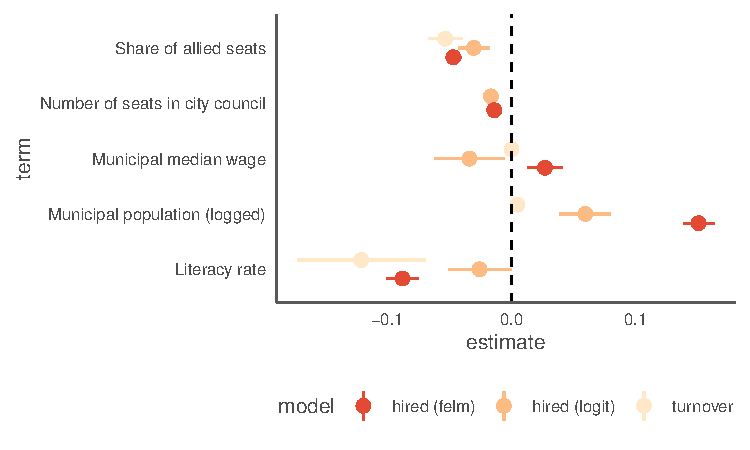
\includegraphics[width=0.6\linewidth]{plots/plot_coalition_coef_mun.pdf}
    \caption{{\bf Political alignment and staff turnover.} A visual representation of results presented in table \ref{tbl:turnover}. All models include year and state fixed effects.}
    \label{fig:coalition_turnover}
\end{figure}

For visual intuition, I present the predicted values for models 4 and 5, respectively the share of hired and dismissed bureaucrats against the share of executive seats in the city council. The reduction in new hires is more pronounced for school principals than teachers, suggesting that exposure to patronage is more concentrated in the leadership positions at the school level. Overall, these results suggest that weaker executive control over the legislature increases patronage, with potentially negative effects for public service delivery in municipalities in Brazil.

\begin{figure}[h]
    \centering
    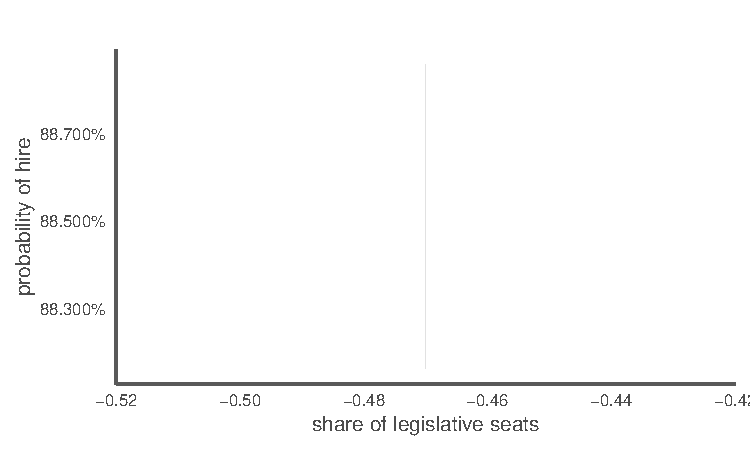
\includegraphics[width=0.6\linewidth]{plots/plot_interactions_logit}
    \caption{\textbf{Differential reductions in patronage in teachers and school principals}. Predicted values for bureaucratic turnover plotted against the proportion of educational staff either hired or fired for any given year against the share of seats controlled by the executive.}
    \label{fig:turnover}
\end{figure}

Finally, I show that the executive-legislative bargain extends to second-term mayors. I subset the data used for the above analysis to only mayors who are reelected, and re-run the previous analyses with the same specification. I find that the results are similar in magnitude and precision to those presented above. This finding suggests that patronage is not motivated solely by reelection concerns. Rather, patronage achieves an important policy goal for incumbent mayors who seek to implement their preferred policy, regardless of whether they are just initiating their mandate or concluding it.

\begin{figure}[h]
    \centering
    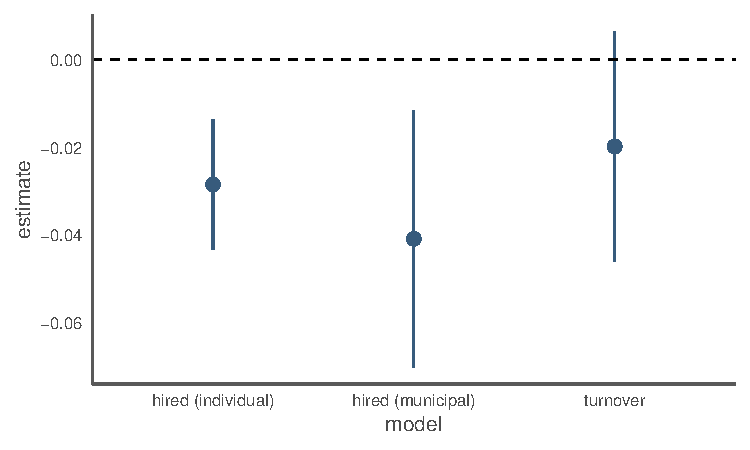
\includegraphics[width=0.6\linewidth]{plots/plot_coalition_coef_mun_second.pdf}
    \caption{\textbf{Patronage continues into the second term.} There is strong evidence that executive-legislative bargains continue into the mayor's second term. All models include a full set of controls, as well as year and state fixed effects.}
\end{figure}

Moving on to characterizing the downstream effects of patronage, I find that teacher and school principal turnover have significant, negative effects on average test scores. These results are robust to alternative specifications of turnover, as well as the use of different quality metrics (SAEB, SPAECE) in our estimations. Table \ref{tbl:student_learning} presents the results of the estimation on SAEB and SPAECE test scores. We present two specifications for turnover. Turnover index measures the amount of turnover in teachers at the school level. Work experience for teachers and school principals serve as an alternative measure of turnover.

\begin{landscape}
    \begin{table}[t]
      \centering
      \footnotesize
      
% Table created by stargazer v.5.2.2 by Marek Hlavac, Harvard University. E-mail: hlavac at fas.harvard.edu
% Date and time: Fri, Jun 12, 2020 - 01:12:19 PM
\begingroup 
\small 
\begin{tabular}{@{\extracolsep{5pt}}lcccccccc} 
\\[-1.8ex]\hline 
\hline \\[-1.8ex] 
 & \multicolumn{8}{c}{Student learning} \\ 
\cline{2-9} 
 & \multicolumn{4}{c}{SAEB test score} & \multicolumn{2}{c}{SPAECE test score} &  &  \\ 
\\[-1.8ex] & (1) & (2) & (3) & (4) & (5) & (6) & (7) & (8)\\ 
\hline \\[-1.8ex] 
 Turnover index & $-$0.073$^{***}$ & $-$0.049$^{***}$ &  &  &  &  & $-$0.054$^{***}$ & $-$0.057$^{***}$ \\ 
  & (0.008) & (0.017) &  &  &  &  & (0.015) & (0.015) \\ 
  Turnover index $\times$ Grade 9 &  &  & $-$0.050$^{***}$ & $-$0.031$^{**}$ &  &  &  &  \\ 
  &  &  & (0.005) & (0.013) &  &  &  &  \\ 
  Teacher experience (2 years) &  &  & 0.028 & $-$0.087$^{**}$ &  &  &  &  \\ 
  &  &  & (0.018) & (0.043) &  &  &  &  \\ 
  Teacher experience (10 years) &  &  &  &  & $-$0.160$^{***}$ & $-$0.120$^{***}$ &  &  \\ 
  &  &  &  &  & (0.006) & (0.014) &  &  \\ 
  School principal experience (2 years) &  &  &  &  & 0.021$^{**}$ & 0.004 &  &  \\ 
  &  &  &  &  & (0.010) & (0.024) &  &  \\ 
  School principal experience (10 years) & 0.004$^{***}$ & 0.003 &  &  &  &  &  &  \\ 
  & (0.001) & (0.003) &  &  &  &  &  &  \\ 
  saeb\_principal\_experienceless than 2 years:grade\_level &  &  & $-$0.003$^{***}$ & $-$0.009$^{***}$ &  &  &  &  \\ 
  &  &  & (0.001) & (0.002) &  &  &  &  \\ 
  saeb\_principal\_experiencemore than 10:grade\_level &  &  & 0.020$^{***}$ & 0.033$^{***}$ &  &  &  &  \\ 
  &  &  & (0.003) & (0.007) &  &  &  &  \\ 
  saeb\_teacher\_work\_schoolless than 2:grade\_level &  &  &  &  & 0.007$^{***}$ & 0.005$^{**}$ &  &  \\ 
  &  &  &  &  & (0.001) & (0.002) &  &  \\ 
  saeb\_teacher\_work\_schoolmore than 10:grade\_level &  &  &  &  & $-$0.002 & $-$0.003 &  &  \\ 
  &  &  &  &  & (0.002) & (0.004) &  &  \\ 
  turnover\_index:grade9 &  &  &  &  &  &  & 0.062$^{***}$ & 0.065$^{***}$ \\ 
  &  &  &  &  &  &  & (0.018) & (0.018) \\ 
 \hline \\[-1.8ex] 
Controls & \_ & \checkmark & \_ & \checkmark & \_ & \checkmark &  &  \\ 
Observations & 165,013 & 26,075 & 1,135,748 & 164,808 & 837,248 & 163,984 & 2,860 & 2,860 \\ 
\hline 
\hline \\[-1.8ex] 
\textit{Note:}  & \multicolumn{8}{r}{$^{*}$p$<$0.1; $^{**}$p$<$0.05; $^{***}$p$<$0.01} \\ 
\end{tabular} 
\endgroup 

      \caption{{\bf Bureaucratic turnover and student learning} Teacher and school principal turnover have a negative effect on student learning. Models 1 and 2 present results for teacher turnover index constructed at the school level. Models 3 and 4 estimate the effect of new teachers and school principals entering the school (less than two years). All models include year and state fixed effects.}
      \label{tbl:student_learning}
    \end{table}
\end{landscape}

I also present the coefficients for the regression exercise above in figure \ref{fig:hlm_mods}. Note that the results are consistent across the board, providing strong evidence that staff turnover has negative downstream consequences for student learning.

\begin{figure}[h]
  \centering
  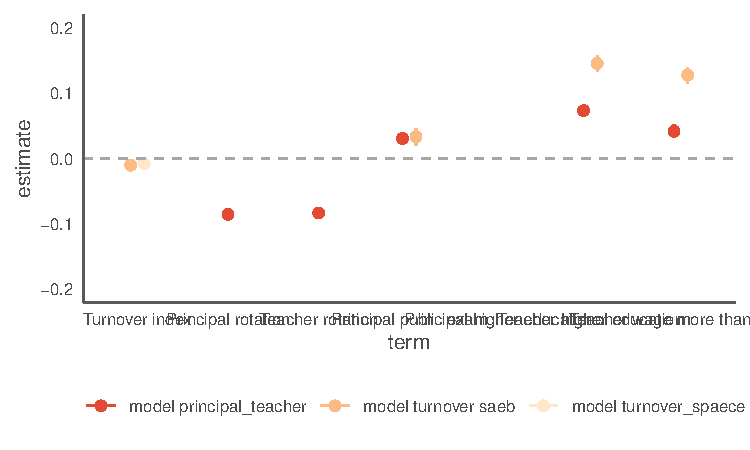
\includegraphics[width=0.6\linewidth]{plots/model_turnover_learning.pdf}
  \caption{{\bf Bureaucratic turnover and student learning} Teacher and school principal turnover have a negative effect on student learning, across different sets of exams (\emph{SAEB} and \emph{SPAECE}). All models include a full set of controls, as well as year and state fixed effects.}
  \label{fig:hlm_mods}
\end{figure}

Finally, I present some evidence of differential returns to patronage, in particular for city councilors. For each position (mayor, city councilor) I estimate the probability of being reelected conditional on the amount of patronage occurred in the first term manda While mayors themselves do not directly benefit from greater patronage, city councilors who are not members of the electoral base of the mayor seem to be negatively affected by patronage appointments into education. The negative consequences of patronage on student learning, however, do not bite, as nayors who deliver a worse quality of education are no less likely to be reelected in the next term.\footnote{See appendix \ref{app:accountability}.}

\begin{figure}[h]
    \centering
    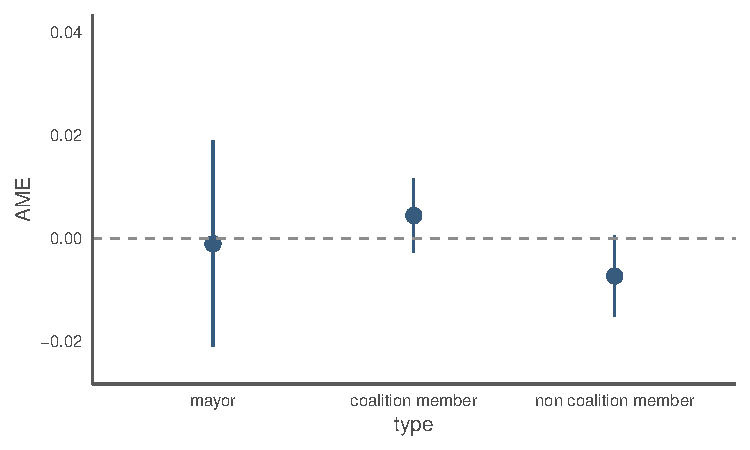
\includegraphics[width=0.6\linewidth]{plots/reelection_marginal_effect_plots.pdf}
    \caption{\textbf{Differential returns to patronage}. Mayors who engage in patronage do not directly benefit from it. Instead, city councilors in the mayoral ally base seem to be benefiting from it at the expense of non-allied city councilors.}
\end{figure}

As a final note, this set of estimations are based on observational data and therefore suffer from well-known concerns of endogeneity. It is in these circumstances that validating causal mechanisms through fieldwork and careful data analysis can increase the validity of a causal claim. In-depth interviews with local actors involved in managing education, as well as the use of different measurements for both educational staff turnover and student learning, provides strong evidence that staff turnover has a negative impact on student learning. Bureaucratic turnover stems from political considerations.

% ## Mechanisms

% The question remains: why do city councilors engage in patronage. Previous studies have found that citizens directly access 

\section{Conclusion}
\label{sec:conclusion}

Improving the quality of education received by children across the world remains a challenge. This paper proposes an analytical framework and estimation strategy to understand the decision-making process behind the administration of educational services in Brazil. In a decentralized context, subnational political actors have a direct say on how educational services are managed, with profound implications for the quality of public services delivered to citizens. These actors interact with bureaucracies and other local elites in complex ways that are only beginning to be mapped.

In this study I theorize and demonstrate that staff turnover stems from the executive's need to garner support from legislators in the city council. This process of coalition building is consolidated through employment offers to city councilors and their constituencies. As the share of seats held by the executive coalition decreases, the costlier it becomes to coopt legislators to support the executive. As a result, the amount of patronage we observe should increase. That is precisely what the data indicates, with teacher turnover increasing in schools, as well as increased hiring and dismissals of teachers and school principals.

This bureaucratic turnover has important consequences for the quality of education delivered in municipalities. I find that turnover has a negative effect on student learning, across a set of specifications for turnover and different evaluation metrics for student learning. The evidence therefore seems to point out that mayors with a weaker hold on the city council resort to greater patronage, with negative consequences for student learning. This set of findings contribute to an emergent literature on the ambiguous consequences of stronger competition in weakly institutionalized contexts \citep{gottlieb_countervailing_2019}.

Future research on patronage and public service delivery would benefit from a clearer treatment of the institutional context in which local political actors operate. Important insights have been derived on executive leaders, but these actors seldom govern alone. Incorporating other local elites paints a more complex and accurate understanding of the strategic considerations taking place in the political management of education, and public services more broadly.

\pagebreak 

\bibliography{dissertation}

\pagebreak

\section*{Appendix}

\subsection{Covariate balance}

\begin{figure}[h]
    \centering
    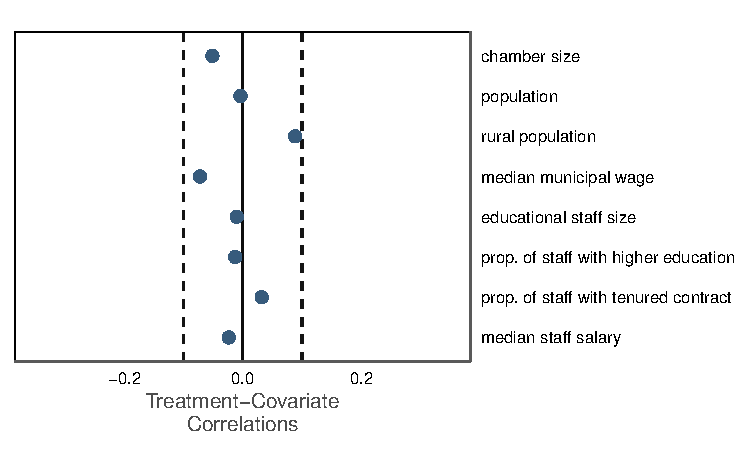
\includegraphics{plots/covariate_balance.pdf}
\end{figure}

\pagebreak

\subsection{Accountability of mayors}
\label{app:accountability}

\begin{figure}[h]
    \centering
    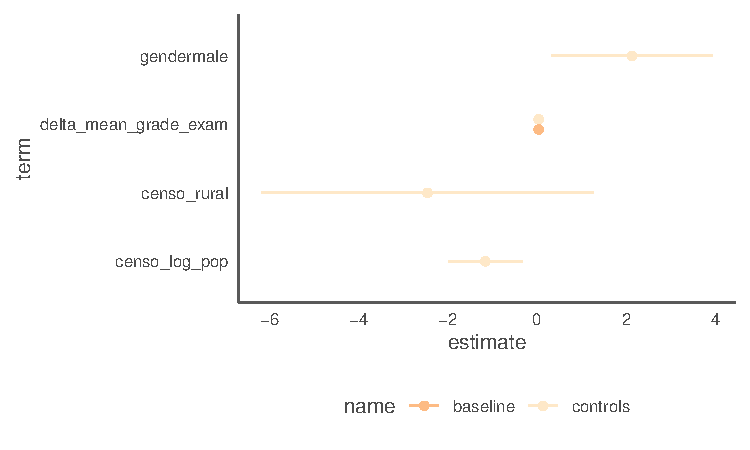
\includegraphics{plots/accountability_fit.pdf}
\end{figure}

\pagebreak

\subsection{Regression Discontinuity Design}

\begin{figure}[h]
    \centering
    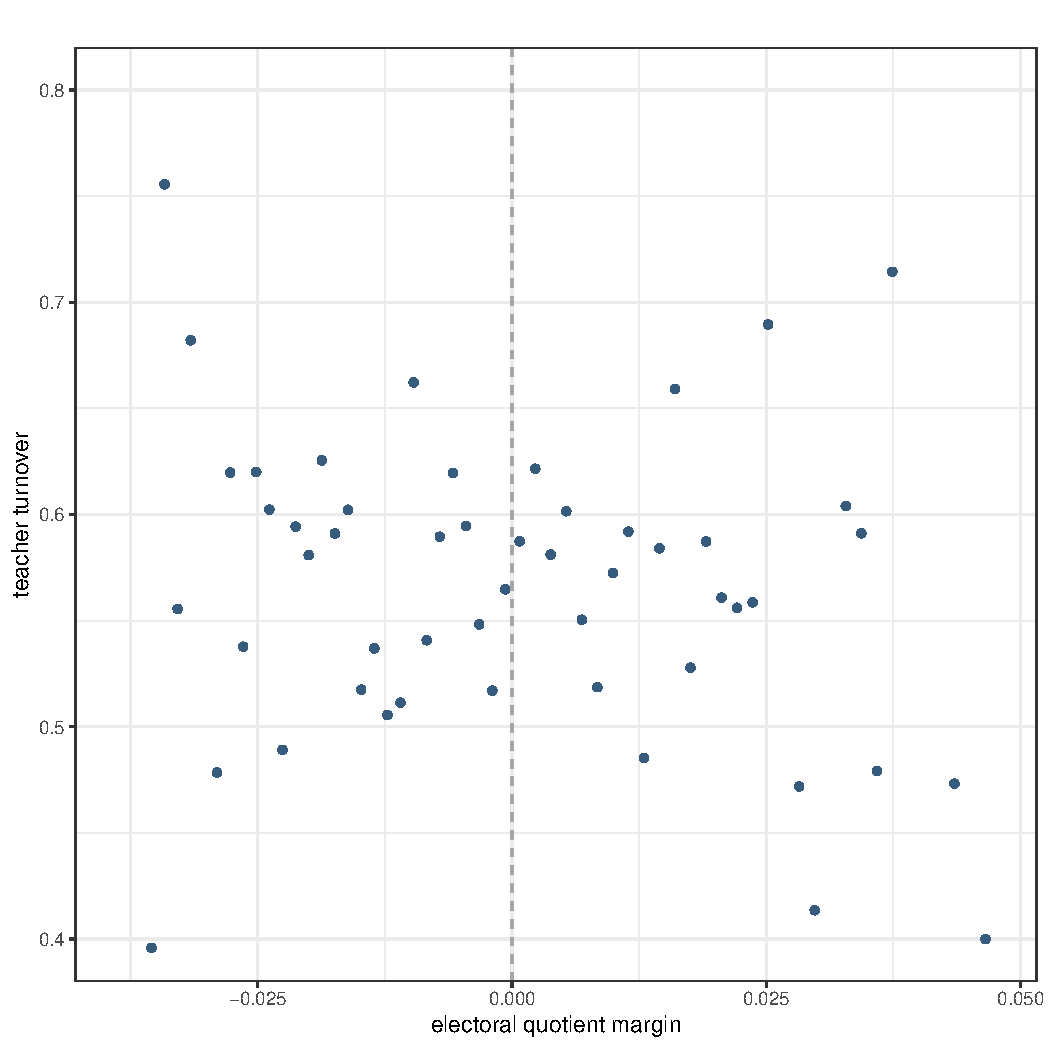
\includegraphics[width=0.7\linewidth]{plots/visual_rdd_legislative_seat_flip.pdf}
\end{figure}

% \blue{plots/balance_hlm}

% ### Staff turnover vs. executive share of legislative seats

% \blue{plots/balance_felm.pdf}

% \pagebreak

\end{document}